% Created by tikzDevice version 0.12.3.2 on 2022-02-15 18:44:33
% !TEX encoding = UTF-8 Unicode
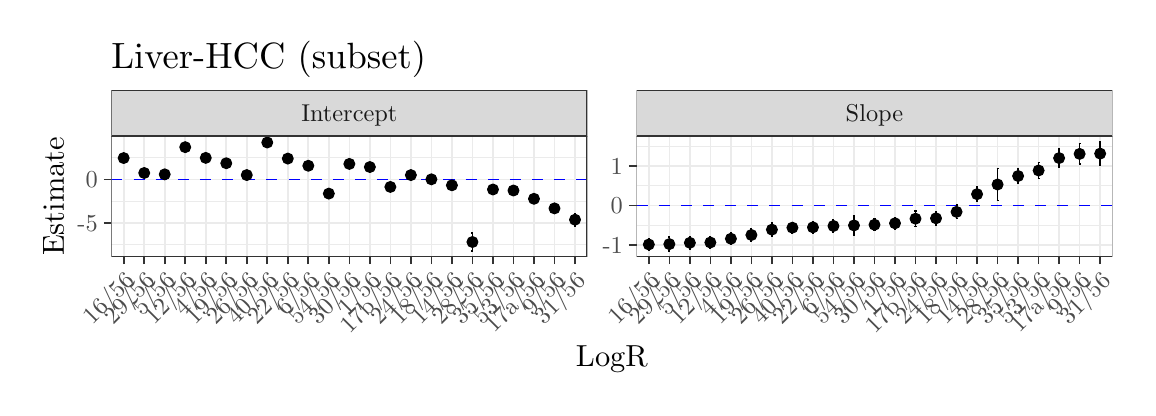
\begin{tikzpicture}[x=1pt,y=1pt]
\definecolor{fillColor}{RGB}{255,255,255}
\path[use as bounding box,fill=fillColor,fill opacity=0.00] (0,0) rectangle (397.48,130.09);
\begin{scope}
\path[clip] (  0.00,  0.00) rectangle (397.48,130.09);
\definecolor{drawColor}{RGB}{255,255,255}
\definecolor{fillColor}{RGB}{255,255,255}

\path[draw=drawColor,line width= 0.6pt,line join=round,line cap=round,fill=fillColor] (  0.00,  0.00) rectangle (397.48,130.09);
\end{scope}
\begin{scope}
\path[clip] ( 30.25, 47.42) rectangle (202.22, 90.86);
\definecolor{fillColor}{RGB}{255,255,255}

\path[fill=fillColor] ( 30.25, 47.42) rectangle (202.22, 90.86);
\definecolor{drawColor}{gray}{0.92}

\path[draw=drawColor,line width= 0.3pt,line join=round] ( 30.25, 51.68) --
	(202.22, 51.68);

\path[draw=drawColor,line width= 0.3pt,line join=round] ( 30.25, 67.41) --
	(202.22, 67.41);

\path[draw=drawColor,line width= 0.3pt,line join=round] ( 30.25, 83.13) --
	(202.22, 83.13);

\path[draw=drawColor,line width= 0.6pt,line join=round] ( 30.25, 59.54) --
	(202.22, 59.54);

\path[draw=drawColor,line width= 0.6pt,line join=round] ( 30.25, 75.27) --
	(202.22, 75.27);

\path[draw=drawColor,line width= 0.6pt,line join=round] ( 34.69, 47.42) --
	( 34.69, 90.86);

\path[draw=drawColor,line width= 0.6pt,line join=round] ( 42.11, 47.42) --
	( 42.11, 90.86);

\path[draw=drawColor,line width= 0.6pt,line join=round] ( 49.52, 47.42) --
	( 49.52, 90.86);

\path[draw=drawColor,line width= 0.6pt,line join=round] ( 56.93, 47.42) --
	( 56.93, 90.86);

\path[draw=drawColor,line width= 0.6pt,line join=round] ( 64.35, 47.42) --
	( 64.35, 90.86);

\path[draw=drawColor,line width= 0.6pt,line join=round] ( 71.76, 47.42) --
	( 71.76, 90.86);

\path[draw=drawColor,line width= 0.6pt,line join=round] ( 79.17, 47.42) --
	( 79.17, 90.86);

\path[draw=drawColor,line width= 0.6pt,line join=round] ( 86.58, 47.42) --
	( 86.58, 90.86);

\path[draw=drawColor,line width= 0.6pt,line join=round] ( 94.00, 47.42) --
	( 94.00, 90.86);

\path[draw=drawColor,line width= 0.6pt,line join=round] (101.41, 47.42) --
	(101.41, 90.86);

\path[draw=drawColor,line width= 0.6pt,line join=round] (108.82, 47.42) --
	(108.82, 90.86);

\path[draw=drawColor,line width= 0.6pt,line join=round] (116.24, 47.42) --
	(116.24, 90.86);

\path[draw=drawColor,line width= 0.6pt,line join=round] (123.65, 47.42) --
	(123.65, 90.86);

\path[draw=drawColor,line width= 0.6pt,line join=round] (131.06, 47.42) --
	(131.06, 90.86);

\path[draw=drawColor,line width= 0.6pt,line join=round] (138.47, 47.42) --
	(138.47, 90.86);

\path[draw=drawColor,line width= 0.6pt,line join=round] (145.89, 47.42) --
	(145.89, 90.86);

\path[draw=drawColor,line width= 0.6pt,line join=round] (153.30, 47.42) --
	(153.30, 90.86);

\path[draw=drawColor,line width= 0.6pt,line join=round] (160.71, 47.42) --
	(160.71, 90.86);

\path[draw=drawColor,line width= 0.6pt,line join=round] (168.13, 47.42) --
	(168.13, 90.86);

\path[draw=drawColor,line width= 0.6pt,line join=round] (175.54, 47.42) --
	(175.54, 90.86);

\path[draw=drawColor,line width= 0.6pt,line join=round] (182.95, 47.42) --
	(182.95, 90.86);

\path[draw=drawColor,line width= 0.6pt,line join=round] (190.36, 47.42) --
	(190.36, 90.86);

\path[draw=drawColor,line width= 0.6pt,line join=round] (197.78, 47.42) --
	(197.78, 90.86);
\definecolor{drawColor}{RGB}{0,0,255}

\path[draw=drawColor,line width= 0.6pt,dash pattern=on 4pt off 4pt ,line join=round] ( 30.25, 75.27) -- (202.22, 75.27);
\definecolor{drawColor}{RGB}{0,0,0}
\definecolor{fillColor}{RGB}{0,0,0}

\path[draw=drawColor,line width= 0.4pt,line join=round,line cap=round,fill=fillColor] (123.65, 79.73) circle (  1.96);

\path[draw=drawColor,line width= 0.4pt,line join=round,line cap=round,fill=fillColor] ( 64.35, 83.04) circle (  1.96);

\path[draw=drawColor,line width= 0.4pt,line join=round,line cap=round,fill=fillColor] ( 49.52, 77.09) circle (  1.96);

\path[draw=drawColor,line width= 0.4pt,line join=round,line cap=round,fill=fillColor] (101.41, 80.19) circle (  1.96);

\path[draw=drawColor,line width= 0.4pt,line join=round,line cap=round,fill=fillColor] (190.36, 64.79) circle (  1.96);

\path[draw=drawColor,line width= 0.4pt,line join=round,line cap=round,fill=fillColor] ( 56.93, 86.91) circle (  1.96);

\path[draw=drawColor,line width= 0.4pt,line join=round,line cap=round,fill=fillColor] (153.30, 73.13) circle (  1.96);

\path[draw=drawColor,line width= 0.4pt,line join=round,line cap=round,fill=fillColor] ( 34.69, 82.98) circle (  1.96);

\path[draw=drawColor,line width= 0.4pt,line join=round,line cap=round,fill=fillColor] (182.95, 68.25) circle (  1.96);

\path[draw=drawColor,line width= 0.4pt,line join=round,line cap=round,fill=fillColor] (131.06, 72.54) circle (  1.96);

\path[draw=drawColor,line width= 0.4pt,line join=round,line cap=round,fill=fillColor] (145.89, 75.29) circle (  1.96);

\path[draw=drawColor,line width= 0.4pt,line join=round,line cap=round,fill=fillColor] ( 71.76, 81.10) circle (  1.96);

\path[draw=drawColor,line width= 0.4pt,line join=round,line cap=round,fill=fillColor] ( 94.00, 82.79) circle (  1.96);

\path[draw=drawColor,line width= 0.4pt,line join=round,line cap=round,fill=fillColor] (138.47, 76.82) circle (  1.96);

\path[draw=drawColor,line width= 0.4pt,line join=round,line cap=round,fill=fillColor] ( 79.17, 76.83) circle (  1.96);

\path[draw=drawColor,line width= 0.4pt,line join=round,line cap=round,fill=fillColor] (160.71, 52.64) circle (  1.96);

\path[draw=drawColor,line width= 0.4pt,line join=round,line cap=round,fill=fillColor] ( 42.11, 77.58) circle (  1.96);

\path[draw=drawColor,line width= 0.4pt,line join=round,line cap=round,fill=fillColor] (116.24, 80.86) circle (  1.96);

\path[draw=drawColor,line width= 0.4pt,line join=round,line cap=round,fill=fillColor] (197.78, 60.70) circle (  1.96);

\path[draw=drawColor,line width= 0.4pt,line join=round,line cap=round,fill=fillColor] (168.13, 71.62) circle (  1.96);

\path[draw=drawColor,line width= 0.4pt,line join=round,line cap=round,fill=fillColor] ( 86.58, 88.60) circle (  1.96);

\path[draw=drawColor,line width= 0.4pt,line join=round,line cap=round,fill=fillColor] (175.54, 71.25) circle (  1.96);

\path[draw=drawColor,line width= 0.4pt,line join=round,line cap=round,fill=fillColor] (108.82, 70.13) circle (  1.96);

\path[draw=drawColor,line width= 0.6pt,line join=round] (123.28, 80.06) --
	(124.02, 80.06);

\path[draw=drawColor,line width= 0.6pt,line join=round] (123.65, 80.06) --
	(123.65, 79.41);

\path[draw=drawColor,line width= 0.6pt,line join=round] (123.28, 79.41) --
	(124.02, 79.41);

\path[draw=drawColor,line width= 0.6pt,line join=round] ( 63.97, 83.39) --
	( 64.72, 83.39);

\path[draw=drawColor,line width= 0.6pt,line join=round] ( 64.35, 83.39) --
	( 64.35, 82.70);

\path[draw=drawColor,line width= 0.6pt,line join=round] ( 63.97, 82.70) --
	( 64.72, 82.70);

\path[draw=drawColor,line width= 0.6pt,line join=round] ( 49.15, 77.74) --
	( 49.89, 77.74);

\path[draw=drawColor,line width= 0.6pt,line join=round] ( 49.52, 77.74) --
	( 49.52, 76.44);

\path[draw=drawColor,line width= 0.6pt,line join=round] ( 49.15, 76.44) --
	( 49.89, 76.44);

\path[draw=drawColor,line width= 0.6pt,line join=round] (101.04, 80.53) --
	(101.78, 80.53);

\path[draw=drawColor,line width= 0.6pt,line join=round] (101.41, 80.53) --
	(101.41, 79.86);

\path[draw=drawColor,line width= 0.6pt,line join=round] (101.04, 79.86) --
	(101.78, 79.86);

\path[draw=drawColor,line width= 0.6pt,line join=round] (189.99, 65.94) --
	(190.73, 65.94);

\path[draw=drawColor,line width= 0.6pt,line join=round] (190.36, 65.94) --
	(190.36, 63.64);

\path[draw=drawColor,line width= 0.6pt,line join=round] (189.99, 63.64) --
	(190.73, 63.64);

\path[draw=drawColor,line width= 0.6pt,line join=round] ( 56.56, 87.20) --
	( 57.30, 87.20);

\path[draw=drawColor,line width= 0.6pt,line join=round] ( 56.93, 87.20) --
	( 56.93, 86.61);

\path[draw=drawColor,line width= 0.6pt,line join=round] ( 56.56, 86.61) --
	( 57.30, 86.61);

\path[draw=drawColor,line width= 0.6pt,line join=round] (152.93, 73.60) --
	(153.67, 73.60);

\path[draw=drawColor,line width= 0.6pt,line join=round] (153.30, 73.60) --
	(153.30, 72.67);

\path[draw=drawColor,line width= 0.6pt,line join=round] (152.93, 72.67) --
	(153.67, 72.67);

\path[draw=drawColor,line width= 0.6pt,line join=round] ( 34.32, 83.29) --
	( 35.06, 83.29);

\path[draw=drawColor,line width= 0.6pt,line join=round] ( 34.69, 83.29) --
	( 34.69, 82.66);

\path[draw=drawColor,line width= 0.6pt,line join=round] ( 34.32, 82.66) --
	( 35.06, 82.66);

\path[draw=drawColor,line width= 0.6pt,line join=round] (182.58, 68.97) --
	(183.32, 68.97);

\path[draw=drawColor,line width= 0.6pt,line join=round] (182.95, 68.97) --
	(182.95, 67.54);

\path[draw=drawColor,line width= 0.6pt,line join=round] (182.58, 67.54) --
	(183.32, 67.54);

\path[draw=drawColor,line width= 0.6pt,line join=round] (130.69, 73.02) --
	(131.43, 73.02);

\path[draw=drawColor,line width= 0.6pt,line join=round] (131.06, 73.02) --
	(131.06, 72.06);

\path[draw=drawColor,line width= 0.6pt,line join=round] (130.69, 72.06) --
	(131.43, 72.06);

\path[draw=drawColor,line width= 0.6pt,line join=round] (145.52, 75.79) --
	(146.26, 75.79);

\path[draw=drawColor,line width= 0.6pt,line join=round] (145.89, 75.79) --
	(145.89, 74.80);

\path[draw=drawColor,line width= 0.6pt,line join=round] (145.52, 74.80) --
	(146.26, 74.80);

\path[draw=drawColor,line width= 0.6pt,line join=round] ( 71.39, 81.41) --
	( 72.13, 81.41);

\path[draw=drawColor,line width= 0.6pt,line join=round] ( 71.76, 81.41) --
	( 71.76, 80.80);

\path[draw=drawColor,line width= 0.6pt,line join=round] ( 71.39, 80.80) --
	( 72.13, 80.80);

\path[draw=drawColor,line width= 0.6pt,line join=round] ( 93.63, 83.08) --
	( 94.37, 83.08);

\path[draw=drawColor,line width= 0.6pt,line join=round] ( 94.00, 83.08) --
	( 94.00, 82.50);

\path[draw=drawColor,line width= 0.6pt,line join=round] ( 93.63, 82.50) --
	( 94.37, 82.50);

\path[draw=drawColor,line width= 0.6pt,line join=round] (138.10, 77.24) --
	(138.84, 77.24);

\path[draw=drawColor,line width= 0.6pt,line join=round] (138.47, 77.24) --
	(138.47, 76.41);

\path[draw=drawColor,line width= 0.6pt,line join=round] (138.10, 76.41) --
	(138.84, 76.41);

\path[draw=drawColor,line width= 0.6pt,line join=round] ( 78.80, 77.30) --
	( 79.54, 77.30);

\path[draw=drawColor,line width= 0.6pt,line join=round] ( 79.17, 77.30) --
	( 79.17, 76.35);

\path[draw=drawColor,line width= 0.6pt,line join=round] ( 78.80, 76.35) --
	( 79.54, 76.35);

\path[draw=drawColor,line width= 0.6pt,line join=round] (160.34, 55.90) --
	(161.08, 55.90);

\path[draw=drawColor,line width= 0.6pt,line join=round] (160.71, 55.90) --
	(160.71, 49.39);

\path[draw=drawColor,line width= 0.6pt,line join=round] (160.34, 49.39) --
	(161.08, 49.39);

\path[draw=drawColor,line width= 0.6pt,line join=round] ( 41.74, 78.00) --
	( 42.48, 78.00);

\path[draw=drawColor,line width= 0.6pt,line join=round] ( 42.11, 78.00) --
	( 42.11, 77.16);

\path[draw=drawColor,line width= 0.6pt,line join=round] ( 41.74, 77.16) --
	( 42.48, 77.16);

\path[draw=drawColor,line width= 0.6pt,line join=round] (115.86, 81.18) --
	(116.61, 81.18);

\path[draw=drawColor,line width= 0.6pt,line join=round] (116.24, 81.18) --
	(116.24, 80.53);

\path[draw=drawColor,line width= 0.6pt,line join=round] (115.86, 80.53) --
	(116.61, 80.53);

\path[draw=drawColor,line width= 0.6pt,line join=round] (197.41, 62.91) --
	(198.15, 62.91);

\path[draw=drawColor,line width= 0.6pt,line join=round] (197.78, 62.91) --
	(197.78, 58.48);

\path[draw=drawColor,line width= 0.6pt,line join=round] (197.41, 58.48) --
	(198.15, 58.48);

\path[draw=drawColor,line width= 0.6pt,line join=round] (167.75, 72.26) --
	(168.50, 72.26);

\path[draw=drawColor,line width= 0.6pt,line join=round] (168.13, 72.26) --
	(168.13, 70.99);

\path[draw=drawColor,line width= 0.6pt,line join=round] (167.75, 70.99) --
	(168.50, 70.99);

\path[draw=drawColor,line width= 0.6pt,line join=round] ( 86.21, 88.88) --
	( 86.95, 88.88);

\path[draw=drawColor,line width= 0.6pt,line join=round] ( 86.58, 88.88) --
	( 86.58, 88.33);

\path[draw=drawColor,line width= 0.6pt,line join=round] ( 86.21, 88.33) --
	( 86.95, 88.33);

\path[draw=drawColor,line width= 0.6pt,line join=round] (175.17, 71.75) --
	(175.91, 71.75);

\path[draw=drawColor,line width= 0.6pt,line join=round] (175.54, 71.75) --
	(175.54, 70.74);

\path[draw=drawColor,line width= 0.6pt,line join=round] (175.17, 70.74) --
	(175.91, 70.74);

\path[draw=drawColor,line width= 0.6pt,line join=round] (108.45, 70.82) --
	(109.19, 70.82);

\path[draw=drawColor,line width= 0.6pt,line join=round] (108.82, 70.82) --
	(108.82, 69.43);

\path[draw=drawColor,line width= 0.6pt,line join=round] (108.45, 69.43) --
	(109.19, 69.43);
\definecolor{drawColor}{gray}{0.20}

\path[draw=drawColor,line width= 0.6pt,line join=round,line cap=round] ( 30.25, 47.42) rectangle (202.22, 90.86);
\end{scope}
\begin{scope}
\path[clip] (220.01, 47.42) rectangle (391.98, 90.86);
\definecolor{fillColor}{RGB}{255,255,255}

\path[fill=fillColor] (220.01, 47.42) rectangle (391.98, 90.86);
\definecolor{drawColor}{gray}{0.92}

\path[draw=drawColor,line width= 0.3pt,line join=round] (220.01, 58.68) --
	(391.98, 58.68);

\path[draw=drawColor,line width= 0.3pt,line join=round] (220.01, 72.96) --
	(391.98, 72.96);

\path[draw=drawColor,line width= 0.3pt,line join=round] (220.01, 87.25) --
	(391.98, 87.25);

\path[draw=drawColor,line width= 0.6pt,line join=round] (220.01, 51.54) --
	(391.98, 51.54);

\path[draw=drawColor,line width= 0.6pt,line join=round] (220.01, 65.82) --
	(391.98, 65.82);

\path[draw=drawColor,line width= 0.6pt,line join=round] (220.01, 80.11) --
	(391.98, 80.11);

\path[draw=drawColor,line width= 0.6pt,line join=round] (224.45, 47.42) --
	(224.45, 90.86);

\path[draw=drawColor,line width= 0.6pt,line join=round] (231.87, 47.42) --
	(231.87, 90.86);

\path[draw=drawColor,line width= 0.6pt,line join=round] (239.28, 47.42) --
	(239.28, 90.86);

\path[draw=drawColor,line width= 0.6pt,line join=round] (246.69, 47.42) --
	(246.69, 90.86);

\path[draw=drawColor,line width= 0.6pt,line join=round] (254.11, 47.42) --
	(254.11, 90.86);

\path[draw=drawColor,line width= 0.6pt,line join=round] (261.52, 47.42) --
	(261.52, 90.86);

\path[draw=drawColor,line width= 0.6pt,line join=round] (268.93, 47.42) --
	(268.93, 90.86);

\path[draw=drawColor,line width= 0.6pt,line join=round] (276.34, 47.42) --
	(276.34, 90.86);

\path[draw=drawColor,line width= 0.6pt,line join=round] (283.76, 47.42) --
	(283.76, 90.86);

\path[draw=drawColor,line width= 0.6pt,line join=round] (291.17, 47.42) --
	(291.17, 90.86);

\path[draw=drawColor,line width= 0.6pt,line join=round] (298.58, 47.42) --
	(298.58, 90.86);

\path[draw=drawColor,line width= 0.6pt,line join=round] (306.00, 47.42) --
	(306.00, 90.86);

\path[draw=drawColor,line width= 0.6pt,line join=round] (313.41, 47.42) --
	(313.41, 90.86);

\path[draw=drawColor,line width= 0.6pt,line join=round] (320.82, 47.42) --
	(320.82, 90.86);

\path[draw=drawColor,line width= 0.6pt,line join=round] (328.23, 47.42) --
	(328.23, 90.86);

\path[draw=drawColor,line width= 0.6pt,line join=round] (335.65, 47.42) --
	(335.65, 90.86);

\path[draw=drawColor,line width= 0.6pt,line join=round] (343.06, 47.42) --
	(343.06, 90.86);

\path[draw=drawColor,line width= 0.6pt,line join=round] (350.47, 47.42) --
	(350.47, 90.86);

\path[draw=drawColor,line width= 0.6pt,line join=round] (357.89, 47.42) --
	(357.89, 90.86);

\path[draw=drawColor,line width= 0.6pt,line join=round] (365.30, 47.42) --
	(365.30, 90.86);

\path[draw=drawColor,line width= 0.6pt,line join=round] (372.71, 47.42) --
	(372.71, 90.86);

\path[draw=drawColor,line width= 0.6pt,line join=round] (380.12, 47.42) --
	(380.12, 90.86);

\path[draw=drawColor,line width= 0.6pt,line join=round] (387.54, 47.42) --
	(387.54, 90.86);
\definecolor{drawColor}{RGB}{0,0,255}

\path[draw=drawColor,line width= 0.6pt,dash pattern=on 4pt off 4pt ,line join=round] (220.01, 65.82) -- (391.98, 65.82);
\definecolor{drawColor}{RGB}{0,0,0}
\definecolor{fillColor}{RGB}{0,0,0}

\path[draw=drawColor,line width= 0.4pt,line join=round,line cap=round,fill=fillColor] (313.41, 59.40) circle (  1.96);

\path[draw=drawColor,line width= 0.4pt,line join=round,line cap=round,fill=fillColor] (254.11, 53.82) circle (  1.96);

\path[draw=drawColor,line width= 0.4pt,line join=round,line cap=round,fill=fillColor] (239.28, 52.35) circle (  1.96);

\path[draw=drawColor,line width= 0.4pt,line join=round,line cap=round,fill=fillColor] (291.17, 58.43) circle (  1.96);

\path[draw=drawColor,line width= 0.4pt,line join=round,line cap=round,fill=fillColor] (380.12, 84.48) circle (  1.96);

\path[draw=drawColor,line width= 0.4pt,line join=round,line cap=round,fill=fillColor] (246.69, 52.46) circle (  1.96);

\path[draw=drawColor,line width= 0.4pt,line join=round,line cap=round,fill=fillColor] (343.06, 69.92) circle (  1.96);

\path[draw=drawColor,line width= 0.4pt,line join=round,line cap=round,fill=fillColor] (224.45, 51.75) circle (  1.96);

\path[draw=drawColor,line width= 0.4pt,line join=round,line cap=round,fill=fillColor] (372.71, 82.97) circle (  1.96);

\path[draw=drawColor,line width= 0.4pt,line join=round,line cap=round,fill=fillColor] (320.82, 61.06) circle (  1.96);

\path[draw=drawColor,line width= 0.4pt,line join=round,line cap=round,fill=fillColor] (335.65, 63.53) circle (  1.96);

\path[draw=drawColor,line width= 0.4pt,line join=round,line cap=round,fill=fillColor] (261.52, 55.17) circle (  1.96);

\path[draw=drawColor,line width= 0.4pt,line join=round,line cap=round,fill=fillColor] (283.76, 57.94) circle (  1.96);

\path[draw=drawColor,line width= 0.4pt,line join=round,line cap=round,fill=fillColor] (328.23, 61.20) circle (  1.96);

\path[draw=drawColor,line width= 0.4pt,line join=round,line cap=round,fill=fillColor] (268.93, 57.11) circle (  1.96);

\path[draw=drawColor,line width= 0.4pt,line join=round,line cap=round,fill=fillColor] (350.47, 73.42) circle (  1.96);

\path[draw=drawColor,line width= 0.4pt,line join=round,line cap=round,fill=fillColor] (231.87, 51.88) circle (  1.96);

\path[draw=drawColor,line width= 0.4pt,line join=round,line cap=round,fill=fillColor] (306.00, 58.88) circle (  1.96);

\path[draw=drawColor,line width= 0.4pt,line join=round,line cap=round,fill=fillColor] (387.54, 84.58) circle (  1.96);

\path[draw=drawColor,line width= 0.4pt,line join=round,line cap=round,fill=fillColor] (357.89, 76.49) circle (  1.96);

\path[draw=drawColor,line width= 0.4pt,line join=round,line cap=round,fill=fillColor] (276.34, 57.82) circle (  1.96);

\path[draw=drawColor,line width= 0.4pt,line join=round,line cap=round,fill=fillColor] (365.30, 78.48) circle (  1.96);

\path[draw=drawColor,line width= 0.4pt,line join=round,line cap=round,fill=fillColor] (298.58, 58.63) circle (  1.96);

\path[draw=drawColor,line width= 0.6pt,line join=round] (313.04, 61.51) --
	(313.78, 61.51);

\path[draw=drawColor,line width= 0.6pt,line join=round] (313.41, 61.51) --
	(313.41, 57.29);

\path[draw=drawColor,line width= 0.6pt,line join=round] (313.04, 57.29) --
	(313.78, 57.29);

\path[draw=drawColor,line width= 0.6pt,line join=round] (253.73, 55.84) --
	(254.48, 55.84);

\path[draw=drawColor,line width= 0.6pt,line join=round] (254.11, 55.84) --
	(254.11, 51.81);

\path[draw=drawColor,line width= 0.6pt,line join=round] (253.73, 51.81) --
	(254.48, 51.81);

\path[draw=drawColor,line width= 0.6pt,line join=round] (238.91, 54.68) --
	(239.65, 54.68);

\path[draw=drawColor,line width= 0.6pt,line join=round] (239.28, 54.68) --
	(239.28, 50.03);

\path[draw=drawColor,line width= 0.6pt,line join=round] (238.91, 50.03) --
	(239.65, 50.03);

\path[draw=drawColor,line width= 0.6pt,line join=round] (290.80, 60.53) --
	(291.54, 60.53);

\path[draw=drawColor,line width= 0.6pt,line join=round] (291.17, 60.53) --
	(291.17, 56.34);

\path[draw=drawColor,line width= 0.6pt,line join=round] (290.80, 56.34) --
	(291.54, 56.34);

\path[draw=drawColor,line width= 0.6pt,line join=round] (379.75, 88.23) --
	(380.50, 88.23);

\path[draw=drawColor,line width= 0.6pt,line join=round] (380.12, 88.23) --
	(380.12, 80.74);

\path[draw=drawColor,line width= 0.6pt,line join=round] (379.75, 80.74) --
	(380.50, 80.74);

\path[draw=drawColor,line width= 0.6pt,line join=round] (246.32, 54.33) --
	(247.06, 54.33);

\path[draw=drawColor,line width= 0.6pt,line join=round] (246.69, 54.33) --
	(246.69, 50.58);

\path[draw=drawColor,line width= 0.6pt,line join=round] (246.32, 50.58) --
	(247.06, 50.58);

\path[draw=drawColor,line width= 0.6pt,line join=round] (342.69, 72.53) --
	(343.43, 72.53);

\path[draw=drawColor,line width= 0.6pt,line join=round] (343.06, 72.53) --
	(343.06, 67.31);

\path[draw=drawColor,line width= 0.6pt,line join=round] (342.69, 67.31) --
	(343.43, 67.31);

\path[draw=drawColor,line width= 0.6pt,line join=round] (224.08, 53.77) --
	(224.82, 53.77);

\path[draw=drawColor,line width= 0.6pt,line join=round] (224.45, 53.77) --
	(224.45, 49.74);

\path[draw=drawColor,line width= 0.6pt,line join=round] (224.08, 49.74) --
	(224.82, 49.74);

\path[draw=drawColor,line width= 0.6pt,line join=round] (372.34, 86.15) --
	(373.08, 86.15);

\path[draw=drawColor,line width= 0.6pt,line join=round] (372.71, 86.15) --
	(372.71, 79.80);

\path[draw=drawColor,line width= 0.6pt,line join=round] (372.34, 79.80) --
	(373.08, 79.80);

\path[draw=drawColor,line width= 0.6pt,line join=round] (320.45, 63.90) --
	(321.19, 63.90);

\path[draw=drawColor,line width= 0.6pt,line join=round] (320.82, 63.90) --
	(320.82, 58.22);

\path[draw=drawColor,line width= 0.6pt,line join=round] (320.45, 58.22) --
	(321.19, 58.22);

\path[draw=drawColor,line width= 0.6pt,line join=round] (335.28, 65.95) --
	(336.02, 65.95);

\path[draw=drawColor,line width= 0.6pt,line join=round] (335.65, 65.95) --
	(335.65, 61.11);

\path[draw=drawColor,line width= 0.6pt,line join=round] (335.28, 61.11) --
	(336.02, 61.11);

\path[draw=drawColor,line width= 0.6pt,line join=round] (261.15, 57.25) --
	(261.89, 57.25);

\path[draw=drawColor,line width= 0.6pt,line join=round] (261.52, 57.25) --
	(261.52, 53.09);

\path[draw=drawColor,line width= 0.6pt,line join=round] (261.15, 53.09) --
	(261.89, 53.09);

\path[draw=drawColor,line width= 0.6pt,line join=round] (283.39, 59.91) --
	(284.13, 59.91);

\path[draw=drawColor,line width= 0.6pt,line join=round] (283.76, 59.91) --
	(283.76, 55.97);

\path[draw=drawColor,line width= 0.6pt,line join=round] (283.39, 55.97) --
	(284.13, 55.97);

\path[draw=drawColor,line width= 0.6pt,line join=round] (327.86, 63.57) --
	(328.60, 63.57);

\path[draw=drawColor,line width= 0.6pt,line join=round] (328.23, 63.57) --
	(328.23, 58.83);

\path[draw=drawColor,line width= 0.6pt,line join=round] (327.86, 58.83) --
	(328.60, 58.83);

\path[draw=drawColor,line width= 0.6pt,line join=round] (268.56, 59.51) --
	(269.30, 59.51);

\path[draw=drawColor,line width= 0.6pt,line join=round] (268.93, 59.51) --
	(268.93, 54.71);

\path[draw=drawColor,line width= 0.6pt,line join=round] (268.56, 54.71) --
	(269.30, 54.71);

\path[draw=drawColor,line width= 0.6pt,line join=round] (350.10, 79.19) --
	(350.84, 79.19);

\path[draw=drawColor,line width= 0.6pt,line join=round] (350.47, 79.19) --
	(350.47, 67.66);

\path[draw=drawColor,line width= 0.6pt,line join=round] (350.10, 67.66) --
	(350.84, 67.66);

\path[draw=drawColor,line width= 0.6pt,line join=round] (231.50, 54.37) --
	(232.24, 54.37);

\path[draw=drawColor,line width= 0.6pt,line join=round] (231.87, 54.37) --
	(231.87, 49.39);

\path[draw=drawColor,line width= 0.6pt,line join=round] (231.50, 49.39) --
	(232.24, 49.39);

\path[draw=drawColor,line width= 0.6pt,line join=round] (305.62, 60.95) --
	(306.37, 60.95);

\path[draw=drawColor,line width= 0.6pt,line join=round] (306.00, 60.95) --
	(306.00, 56.81);

\path[draw=drawColor,line width= 0.6pt,line join=round] (305.62, 56.81) --
	(306.37, 56.81);

\path[draw=drawColor,line width= 0.6pt,line join=round] (387.17, 88.88) --
	(387.91, 88.88);

\path[draw=drawColor,line width= 0.6pt,line join=round] (387.54, 88.88) --
	(387.54, 80.28);

\path[draw=drawColor,line width= 0.6pt,line join=round] (387.17, 80.28) --
	(387.91, 80.28);

\path[draw=drawColor,line width= 0.6pt,line join=round] (357.52, 79.06) --
	(358.26, 79.06);

\path[draw=drawColor,line width= 0.6pt,line join=round] (357.89, 79.06) --
	(357.89, 73.93);

\path[draw=drawColor,line width= 0.6pt,line join=round] (357.52, 73.93) --
	(358.26, 73.93);

\path[draw=drawColor,line width= 0.6pt,line join=round] (275.97, 59.66) --
	(276.71, 59.66);

\path[draw=drawColor,line width= 0.6pt,line join=round] (276.34, 59.66) --
	(276.34, 55.98);

\path[draw=drawColor,line width= 0.6pt,line join=round] (275.97, 55.98) --
	(276.71, 55.98);

\path[draw=drawColor,line width= 0.6pt,line join=round] (364.93, 81.32) --
	(365.67, 81.32);

\path[draw=drawColor,line width= 0.6pt,line join=round] (365.30, 81.32) --
	(365.30, 75.64);

\path[draw=drawColor,line width= 0.6pt,line join=round] (364.93, 75.64) --
	(365.67, 75.64);

\path[draw=drawColor,line width= 0.6pt,line join=round] (298.21, 62.00) --
	(298.95, 62.00);

\path[draw=drawColor,line width= 0.6pt,line join=round] (298.58, 62.00) --
	(298.58, 55.26);

\path[draw=drawColor,line width= 0.6pt,line join=round] (298.21, 55.26) --
	(298.95, 55.26);
\definecolor{drawColor}{gray}{0.20}

\path[draw=drawColor,line width= 0.6pt,line join=round,line cap=round] (220.01, 47.42) rectangle (391.98, 90.86);
\end{scope}
\begin{scope}
\path[clip] ( 30.25, 90.86) rectangle (202.22,107.43);
\definecolor{drawColor}{gray}{0.20}
\definecolor{fillColor}{gray}{0.85}

\path[draw=drawColor,line width= 0.6pt,line join=round,line cap=round,fill=fillColor] ( 30.25, 90.86) rectangle (202.22,107.43);
\definecolor{drawColor}{gray}{0.10}

\node[text=drawColor,anchor=base,inner sep=0pt, outer sep=0pt, scale=  0.88] at (116.24, 96.11) {Intercept};
\end{scope}
\begin{scope}
\path[clip] (220.01, 90.86) rectangle (391.98,107.43);
\definecolor{drawColor}{gray}{0.20}
\definecolor{fillColor}{gray}{0.85}

\path[draw=drawColor,line width= 0.6pt,line join=round,line cap=round,fill=fillColor] (220.01, 90.86) rectangle (391.98,107.43);
\definecolor{drawColor}{gray}{0.10}

\node[text=drawColor,anchor=base,inner sep=0pt, outer sep=0pt, scale=  0.88] at (306.00, 96.11) {Slope};
\end{scope}
\begin{scope}
\path[clip] (  0.00,  0.00) rectangle (397.48,130.09);
\definecolor{drawColor}{gray}{0.20}

\path[draw=drawColor,line width= 0.6pt,line join=round] ( 34.69, 44.67) --
	( 34.69, 47.42);

\path[draw=drawColor,line width= 0.6pt,line join=round] ( 42.11, 44.67) --
	( 42.11, 47.42);

\path[draw=drawColor,line width= 0.6pt,line join=round] ( 49.52, 44.67) --
	( 49.52, 47.42);

\path[draw=drawColor,line width= 0.6pt,line join=round] ( 56.93, 44.67) --
	( 56.93, 47.42);

\path[draw=drawColor,line width= 0.6pt,line join=round] ( 64.35, 44.67) --
	( 64.35, 47.42);

\path[draw=drawColor,line width= 0.6pt,line join=round] ( 71.76, 44.67) --
	( 71.76, 47.42);

\path[draw=drawColor,line width= 0.6pt,line join=round] ( 79.17, 44.67) --
	( 79.17, 47.42);

\path[draw=drawColor,line width= 0.6pt,line join=round] ( 86.58, 44.67) --
	( 86.58, 47.42);

\path[draw=drawColor,line width= 0.6pt,line join=round] ( 94.00, 44.67) --
	( 94.00, 47.42);

\path[draw=drawColor,line width= 0.6pt,line join=round] (101.41, 44.67) --
	(101.41, 47.42);

\path[draw=drawColor,line width= 0.6pt,line join=round] (108.82, 44.67) --
	(108.82, 47.42);

\path[draw=drawColor,line width= 0.6pt,line join=round] (116.24, 44.67) --
	(116.24, 47.42);

\path[draw=drawColor,line width= 0.6pt,line join=round] (123.65, 44.67) --
	(123.65, 47.42);

\path[draw=drawColor,line width= 0.6pt,line join=round] (131.06, 44.67) --
	(131.06, 47.42);

\path[draw=drawColor,line width= 0.6pt,line join=round] (138.47, 44.67) --
	(138.47, 47.42);

\path[draw=drawColor,line width= 0.6pt,line join=round] (145.89, 44.67) --
	(145.89, 47.42);

\path[draw=drawColor,line width= 0.6pt,line join=round] (153.30, 44.67) --
	(153.30, 47.42);

\path[draw=drawColor,line width= 0.6pt,line join=round] (160.71, 44.67) --
	(160.71, 47.42);

\path[draw=drawColor,line width= 0.6pt,line join=round] (168.13, 44.67) --
	(168.13, 47.42);

\path[draw=drawColor,line width= 0.6pt,line join=round] (175.54, 44.67) --
	(175.54, 47.42);

\path[draw=drawColor,line width= 0.6pt,line join=round] (182.95, 44.67) --
	(182.95, 47.42);

\path[draw=drawColor,line width= 0.6pt,line join=round] (190.36, 44.67) --
	(190.36, 47.42);

\path[draw=drawColor,line width= 0.6pt,line join=round] (197.78, 44.67) --
	(197.78, 47.42);
\end{scope}
\begin{scope}
\path[clip] (  0.00,  0.00) rectangle (397.48,130.09);
\definecolor{drawColor}{gray}{0.30}

\node[text=drawColor,rotate= 45.00,anchor=base east,inner sep=0pt, outer sep=0pt, scale=  0.88] at ( 38.98, 38.18) {16/56};

\node[text=drawColor,rotate= 45.00,anchor=base east,inner sep=0pt, outer sep=0pt, scale=  0.88] at ( 46.39, 38.18) {29/56};

\node[text=drawColor,rotate= 45.00,anchor=base east,inner sep=0pt, outer sep=0pt, scale=  0.88] at ( 53.81, 38.18) {5/56};

\node[text=drawColor,rotate= 45.00,anchor=base east,inner sep=0pt, outer sep=0pt, scale=  0.88] at ( 61.22, 38.18) {12/56};

\node[text=drawColor,rotate= 45.00,anchor=base east,inner sep=0pt, outer sep=0pt, scale=  0.88] at ( 68.63, 38.18) {4/56};

\node[text=drawColor,rotate= 45.00,anchor=base east,inner sep=0pt, outer sep=0pt, scale=  0.88] at ( 76.04, 38.18) {19/56};

\node[text=drawColor,rotate= 45.00,anchor=base east,inner sep=0pt, outer sep=0pt, scale=  0.88] at ( 83.46, 38.18) {26/56};

\node[text=drawColor,rotate= 45.00,anchor=base east,inner sep=0pt, outer sep=0pt, scale=  0.88] at ( 90.87, 38.18) {40/56};

\node[text=drawColor,rotate= 45.00,anchor=base east,inner sep=0pt, outer sep=0pt, scale=  0.88] at ( 98.28, 38.18) {22/56};

\node[text=drawColor,rotate= 45.00,anchor=base east,inner sep=0pt, outer sep=0pt, scale=  0.88] at (105.70, 38.18) {6/56};

\node[text=drawColor,rotate= 45.00,anchor=base east,inner sep=0pt, outer sep=0pt, scale=  0.88] at (113.11, 38.18) {54/56};

\node[text=drawColor,rotate= 45.00,anchor=base east,inner sep=0pt, outer sep=0pt, scale=  0.88] at (120.52, 38.18) {30/56};

\node[text=drawColor,rotate= 45.00,anchor=base east,inner sep=0pt, outer sep=0pt, scale=  0.88] at (127.93, 38.18) {1/56};

\node[text=drawColor,rotate= 45.00,anchor=base east,inner sep=0pt, outer sep=0pt, scale=  0.88] at (135.35, 38.18) {17b/56};

\node[text=drawColor,rotate= 45.00,anchor=base east,inner sep=0pt, outer sep=0pt, scale=  0.88] at (142.76, 38.18) {24/56};

\node[text=drawColor,rotate= 45.00,anchor=base east,inner sep=0pt, outer sep=0pt, scale=  0.88] at (150.17, 38.18) {18/56};

\node[text=drawColor,rotate= 45.00,anchor=base east,inner sep=0pt, outer sep=0pt, scale=  0.88] at (157.59, 38.18) {14/56};

\node[text=drawColor,rotate= 45.00,anchor=base east,inner sep=0pt, outer sep=0pt, scale=  0.88] at (165.00, 38.18) {28/56};

\node[text=drawColor,rotate= 45.00,anchor=base east,inner sep=0pt, outer sep=0pt, scale=  0.88] at (172.41, 38.18) {35/56};

\node[text=drawColor,rotate= 45.00,anchor=base east,inner sep=0pt, outer sep=0pt, scale=  0.88] at (179.82, 38.18) {53/56};

\node[text=drawColor,rotate= 45.00,anchor=base east,inner sep=0pt, outer sep=0pt, scale=  0.88] at (187.24, 38.18) {17a/56};

\node[text=drawColor,rotate= 45.00,anchor=base east,inner sep=0pt, outer sep=0pt, scale=  0.88] at (194.65, 38.18) {9/56};

\node[text=drawColor,rotate= 45.00,anchor=base east,inner sep=0pt, outer sep=0pt, scale=  0.88] at (202.06, 38.18) {31/56};
\end{scope}
\begin{scope}
\path[clip] (  0.00,  0.00) rectangle (397.48,130.09);
\definecolor{drawColor}{gray}{0.20}

\path[draw=drawColor,line width= 0.6pt,line join=round] (224.45, 44.67) --
	(224.45, 47.42);

\path[draw=drawColor,line width= 0.6pt,line join=round] (231.87, 44.67) --
	(231.87, 47.42);

\path[draw=drawColor,line width= 0.6pt,line join=round] (239.28, 44.67) --
	(239.28, 47.42);

\path[draw=drawColor,line width= 0.6pt,line join=round] (246.69, 44.67) --
	(246.69, 47.42);

\path[draw=drawColor,line width= 0.6pt,line join=round] (254.11, 44.67) --
	(254.11, 47.42);

\path[draw=drawColor,line width= 0.6pt,line join=round] (261.52, 44.67) --
	(261.52, 47.42);

\path[draw=drawColor,line width= 0.6pt,line join=round] (268.93, 44.67) --
	(268.93, 47.42);

\path[draw=drawColor,line width= 0.6pt,line join=round] (276.34, 44.67) --
	(276.34, 47.42);

\path[draw=drawColor,line width= 0.6pt,line join=round] (283.76, 44.67) --
	(283.76, 47.42);

\path[draw=drawColor,line width= 0.6pt,line join=round] (291.17, 44.67) --
	(291.17, 47.42);

\path[draw=drawColor,line width= 0.6pt,line join=round] (298.58, 44.67) --
	(298.58, 47.42);

\path[draw=drawColor,line width= 0.6pt,line join=round] (306.00, 44.67) --
	(306.00, 47.42);

\path[draw=drawColor,line width= 0.6pt,line join=round] (313.41, 44.67) --
	(313.41, 47.42);

\path[draw=drawColor,line width= 0.6pt,line join=round] (320.82, 44.67) --
	(320.82, 47.42);

\path[draw=drawColor,line width= 0.6pt,line join=round] (328.23, 44.67) --
	(328.23, 47.42);

\path[draw=drawColor,line width= 0.6pt,line join=round] (335.65, 44.67) --
	(335.65, 47.42);

\path[draw=drawColor,line width= 0.6pt,line join=round] (343.06, 44.67) --
	(343.06, 47.42);

\path[draw=drawColor,line width= 0.6pt,line join=round] (350.47, 44.67) --
	(350.47, 47.42);

\path[draw=drawColor,line width= 0.6pt,line join=round] (357.89, 44.67) --
	(357.89, 47.42);

\path[draw=drawColor,line width= 0.6pt,line join=round] (365.30, 44.67) --
	(365.30, 47.42);

\path[draw=drawColor,line width= 0.6pt,line join=round] (372.71, 44.67) --
	(372.71, 47.42);

\path[draw=drawColor,line width= 0.6pt,line join=round] (380.12, 44.67) --
	(380.12, 47.42);

\path[draw=drawColor,line width= 0.6pt,line join=round] (387.54, 44.67) --
	(387.54, 47.42);
\end{scope}
\begin{scope}
\path[clip] (  0.00,  0.00) rectangle (397.48,130.09);
\definecolor{drawColor}{gray}{0.30}

\node[text=drawColor,rotate= 45.00,anchor=base east,inner sep=0pt, outer sep=0pt, scale=  0.88] at (228.74, 38.18) {16/56};

\node[text=drawColor,rotate= 45.00,anchor=base east,inner sep=0pt, outer sep=0pt, scale=  0.88] at (236.15, 38.18) {29/56};

\node[text=drawColor,rotate= 45.00,anchor=base east,inner sep=0pt, outer sep=0pt, scale=  0.88] at (243.57, 38.18) {5/56};

\node[text=drawColor,rotate= 45.00,anchor=base east,inner sep=0pt, outer sep=0pt, scale=  0.88] at (250.98, 38.18) {12/56};

\node[text=drawColor,rotate= 45.00,anchor=base east,inner sep=0pt, outer sep=0pt, scale=  0.88] at (258.39, 38.18) {4/56};

\node[text=drawColor,rotate= 45.00,anchor=base east,inner sep=0pt, outer sep=0pt, scale=  0.88] at (265.80, 38.18) {19/56};

\node[text=drawColor,rotate= 45.00,anchor=base east,inner sep=0pt, outer sep=0pt, scale=  0.88] at (273.22, 38.18) {26/56};

\node[text=drawColor,rotate= 45.00,anchor=base east,inner sep=0pt, outer sep=0pt, scale=  0.88] at (280.63, 38.18) {40/56};

\node[text=drawColor,rotate= 45.00,anchor=base east,inner sep=0pt, outer sep=0pt, scale=  0.88] at (288.04, 38.18) {22/56};

\node[text=drawColor,rotate= 45.00,anchor=base east,inner sep=0pt, outer sep=0pt, scale=  0.88] at (295.46, 38.18) {6/56};

\node[text=drawColor,rotate= 45.00,anchor=base east,inner sep=0pt, outer sep=0pt, scale=  0.88] at (302.87, 38.18) {54/56};

\node[text=drawColor,rotate= 45.00,anchor=base east,inner sep=0pt, outer sep=0pt, scale=  0.88] at (310.28, 38.18) {30/56};

\node[text=drawColor,rotate= 45.00,anchor=base east,inner sep=0pt, outer sep=0pt, scale=  0.88] at (317.69, 38.18) {1/56};

\node[text=drawColor,rotate= 45.00,anchor=base east,inner sep=0pt, outer sep=0pt, scale=  0.88] at (325.11, 38.18) {17b/56};

\node[text=drawColor,rotate= 45.00,anchor=base east,inner sep=0pt, outer sep=0pt, scale=  0.88] at (332.52, 38.18) {24/56};

\node[text=drawColor,rotate= 45.00,anchor=base east,inner sep=0pt, outer sep=0pt, scale=  0.88] at (339.93, 38.18) {18/56};

\node[text=drawColor,rotate= 45.00,anchor=base east,inner sep=0pt, outer sep=0pt, scale=  0.88] at (347.35, 38.18) {14/56};

\node[text=drawColor,rotate= 45.00,anchor=base east,inner sep=0pt, outer sep=0pt, scale=  0.88] at (354.76, 38.18) {28/56};

\node[text=drawColor,rotate= 45.00,anchor=base east,inner sep=0pt, outer sep=0pt, scale=  0.88] at (362.17, 38.18) {35/56};

\node[text=drawColor,rotate= 45.00,anchor=base east,inner sep=0pt, outer sep=0pt, scale=  0.88] at (369.58, 38.18) {53/56};

\node[text=drawColor,rotate= 45.00,anchor=base east,inner sep=0pt, outer sep=0pt, scale=  0.88] at (377.00, 38.18) {17a/56};

\node[text=drawColor,rotate= 45.00,anchor=base east,inner sep=0pt, outer sep=0pt, scale=  0.88] at (384.41, 38.18) {9/56};

\node[text=drawColor,rotate= 45.00,anchor=base east,inner sep=0pt, outer sep=0pt, scale=  0.88] at (391.82, 38.18) {31/56};
\end{scope}
\begin{scope}
\path[clip] (  0.00,  0.00) rectangle (397.48,130.09);
\definecolor{drawColor}{gray}{0.30}

\node[text=drawColor,anchor=base east,inner sep=0pt, outer sep=0pt, scale=  0.88] at (215.06, 48.51) {-1};

\node[text=drawColor,anchor=base east,inner sep=0pt, outer sep=0pt, scale=  0.88] at (215.06, 62.79) {0};

\node[text=drawColor,anchor=base east,inner sep=0pt, outer sep=0pt, scale=  0.88] at (215.06, 77.08) {1};
\end{scope}
\begin{scope}
\path[clip] (  0.00,  0.00) rectangle (397.48,130.09);
\definecolor{drawColor}{gray}{0.20}

\path[draw=drawColor,line width= 0.6pt,line join=round] (217.26, 51.54) --
	(220.01, 51.54);

\path[draw=drawColor,line width= 0.6pt,line join=round] (217.26, 65.82) --
	(220.01, 65.82);

\path[draw=drawColor,line width= 0.6pt,line join=round] (217.26, 80.11) --
	(220.01, 80.11);
\end{scope}
\begin{scope}
\path[clip] (  0.00,  0.00) rectangle (397.48,130.09);
\definecolor{drawColor}{gray}{0.30}

\node[text=drawColor,anchor=base east,inner sep=0pt, outer sep=0pt, scale=  0.88] at ( 25.30, 56.51) {-5};

\node[text=drawColor,anchor=base east,inner sep=0pt, outer sep=0pt, scale=  0.88] at ( 25.30, 72.24) {0};
\end{scope}
\begin{scope}
\path[clip] (  0.00,  0.00) rectangle (397.48,130.09);
\definecolor{drawColor}{gray}{0.20}

\path[draw=drawColor,line width= 0.6pt,line join=round] ( 27.50, 59.54) --
	( 30.25, 59.54);

\path[draw=drawColor,line width= 0.6pt,line join=round] ( 27.50, 75.27) --
	( 30.25, 75.27);
\end{scope}
\begin{scope}
\path[clip] (  0.00,  0.00) rectangle (397.48,130.09);
\definecolor{drawColor}{RGB}{0,0,0}

\node[text=drawColor,anchor=base,inner sep=0pt, outer sep=0pt, scale=  1.10] at (211.12,  7.64) {LogR};
\end{scope}
\begin{scope}
\path[clip] (  0.00,  0.00) rectangle (397.48,130.09);
\definecolor{drawColor}{RGB}{0,0,0}

\node[text=drawColor,rotate= 90.00,anchor=base,inner sep=0pt, outer sep=0pt, scale=  1.10] at ( 13.08, 69.14) {Estimate};
\end{scope}
\begin{scope}
\path[clip] (  0.00,  0.00) rectangle (397.48,130.09);
\definecolor{drawColor}{RGB}{0,0,0}

\node[text=drawColor,anchor=base west,inner sep=0pt, outer sep=0pt, scale=  1.32] at ( 30.25,115.49) {Liver-HCC (subset)};
\end{scope}
\end{tikzpicture}
